\section{Introduction}

Previous works on cloudlets~\cite{Satya2009Case,Ha2013Impact}, one of the earliest incarnation of edge computing, enable small data-centers at the edge of the Internet. 
Many futuristic applications become viable with these clusters that are only one wireless hop away. 
One of the most promising genres of these emerging applications is human-in-the-loop applications such as wearable cognitive assistance~\cite{Ha2014Towards}. 

In these applications, sensor data, for example video and audio, are continuously streamed to a cloudlet, where they are analyzed in realtime in order to assist users to complete a particular task. 
Researchers have built prototypes of these applications to help users assemble LEGO models and IKEA furniture, and even learn how to play ping-pong~\cite{Satya2009Case,Chen2015Early}.
% In general, all human-in-the-loop applications capture in some form user and environment information and typically leverage compute-intensive algorithms to analyze the data in order to provide feedback to the user.
% On the side of the sensory input, typically video, but also audio as well as further user-related data (like orientation and movement) is captured.
% This  data is forwarded to the processing unit where the first step is usually to run detection algorithms on the sensory input.
% In case of a positive result from the detection, the next step is then the generation of feedback to be sent back to the user.

Cognitive assistance applications are highly interactive. 
Feedback is sent back to the user once the application detects interesting events, for example, when the user places the wrong LEGO block on the model.
% For this the detected features are put into the context of the specific application and its task model (for instance for assistance applications a comparison to the current task goal and potentially the required step towards the next task goal) which then leads potentially to feedback that has to be provided to the user.
% Thus, the next step is to generate this feedback and forward this back to the user, where it is exposed to the user.
%, as shown in Figure~\ref{fig:app-pipeline}.
%, from which on a user takes further actions, triggering the next loop of the application. 
The feedback loop is then repeated until the user finishes the task.
It is important to note that not all sensory input triggers feedback.
Take for instance, an application which relies on image recognition.
Inevitably, some frames are going to receive confidence values below a set threshold from the image recognition algorithms, and thus do not generate feedback.
We will refer to these inputs as \emph{feedback-poor}, and conversely, refer to inputs which do generate feedback as \emph{feedback-rich}.

% In the following, we distinguish between input (i.e. frames) triggering feedback whereas frames for which no new state is detected are referred to as ones that do not provide feedback (i.e. frames without feedback). 

These principles result in the following characteristics of human-in-the-loop applications powered by edge computing:

\begin{description}[labelindent=\parindent, listparindent=\parindent, style=unboxed, leftmargin=0cm]
	\item[Latency Sensitive:] Given their tight interaction with the physical world, the quality of human-in-the-loop applications is determined by the latencies experienced by users. 
    These applications are different from conventional mobile applications by the low latency requirements inherent to the applications themselves~\cite{Suzuki2016Vehicle,Chen2017Empirical}. 
    For example, consider a Ping-Pong Assistance application that instructs a user where to hit a ball -- any instruction delivered after the user has made a hit is useless.
  Hence, the average and the distribution of end-to-end latency, in particular for \emph{feedback-rich} inputs, can serve as good metrics for a benchmark tool. 
% Previous work has shown that offload to cloudlet reduces 100ms to 200ms in end-to-end latency from offload to the cloud \cite{Suzuki,Chen:AnEmpiricalStudyOfLatency}.
% Thus, the low latency benefits provided by cloudlets distinguish human-in-the-loop applications from conventional mobile or web applications. 
% Therefore, low latency is a salient characteristic of cloudlet-enabled applications.
	
    \item[Compute Intensive:] Cognitive Assistance applications aim to enhance the cognitive capabilities of users, and are thus compute intensive as well due to widespread use of the state-of-art computer vision and machine learning algorithms, particularly \acp{DNN}. 
    Although mobile devices are becoming increasingly powerful, the gap between mobile and static elements continues to exist~\cite{Flinn2012Cyber}. 
    While state-of-the-art DNN object detectors can run at more than 20 \acs{FPS} on a server \acs{GPU}, their performances are much worse on mobile \acsp{GPU} - some models cannot even be loaded due to memory constraints. 
    Cloudlet-based applications overcome these challenges by offloading the computation. 
%    Offloading makes sense when the computation is intensive or special hardwares are needed. 

\end{description}


% Experimentally, it has been shown \cite{Chen:AnEmpiricalStudyOfLatency} that human-in-the-loop applications are perceived within one of three coarse quality-of-experience ranges: Flawless, impaired and useless. If such an application experiences a round-trip delay below a certain threshold $\tau_1$, further improvememt of the round-trip delay does not lead to a better perceived quality of experience (at least with respect to subjective user experience). The delay range below threshold $\tau_1$ is hence referred to as flawless. Furthermore, there is a second round-trip delay threshold $\tau_2$ which represents a cut-off beyond which a human-in-the-loop application is perceived as useless, i.e. an assistance application can not provide any help due to the delays in this case. The range in between $\tau_1$ and $\tau_2$ is generally perceived as a range where the application can still be operated but a degradation in the quality of experience is perceived, which degrades with the absolute value of the round-trip time within the given range. 
% In terms of absolute values, $\tau_1$ and $\tau_2$ are generally application-dependent while spanning from a few tens to a few hundreds of milliseconds.
% Finally, note that for the round-trip times in particular the sensory input triggering feedback is of key relevance for the perceived quality-of-experience.

Benchmarking infrastructures for these human-in-the-loop applications is challenging -- the main issue arises from the involvement of humans. % in the application.
Applications' execution path and resource utilization vary among users. 
For example, in a task guidance application, the reaction speed of the human to a new instruction governs the inter-arrival time of the next \emph{feedback-rich} input.
Furthermore, large scale evaluation of these applications require the involvement of many human users. % and provide feedback.
Both these aspects significantly limit experimental studies that could be done to improve architectures, algorithms, and protocols due to costs, efforts as well as reproducibility.

\section{The Measurement Framework}\label{sec:framework}

% \begin{figure*}[t]
% 	\centering
%     \begin{minipage}{.7\linewidth}
%     	\centering
%         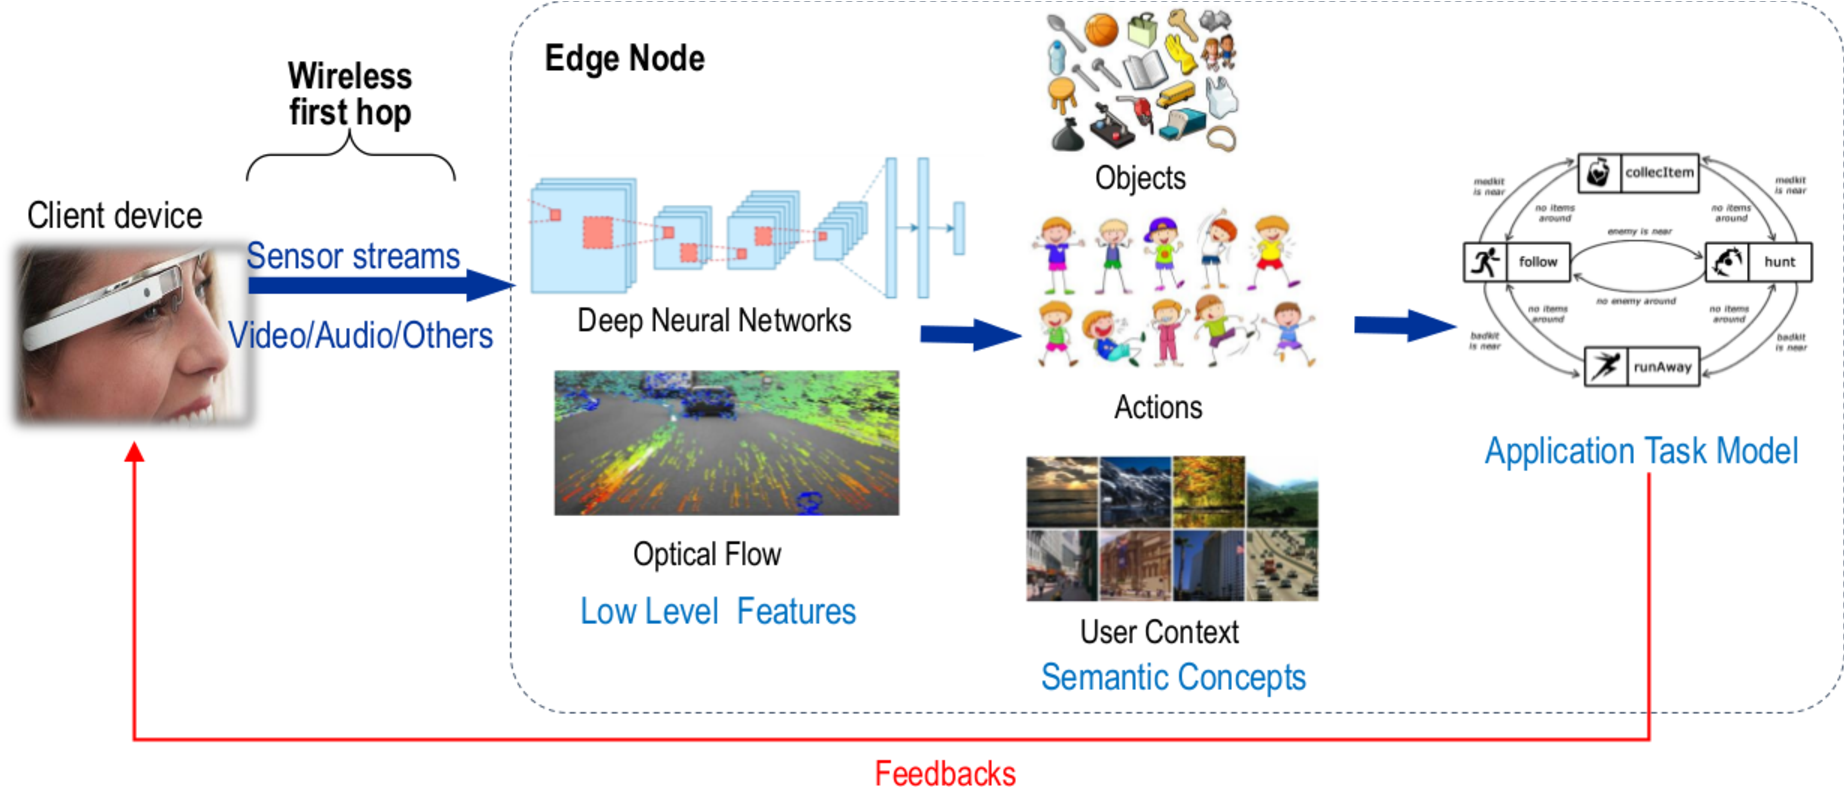
\includegraphics[width=.9\textwidth]{img/app_pipeline.pdf}
%         \captionof{figure}{Generic Human-in-the-loop Application Pipeline}
%         \label{fig:app-pipeline}
%     \end{minipage}%
% 	\begin{minipage}{.3\linewidth}
%     	\centering
% 		\includegraphics[width=\linewidth]{img/TraceReplay_GenArch}
%         \captionof{figure}{General architecture of the benchmarking suite.}
% 		\label{fig:TraceReplayArch}
% 	\end{minipage}
% \end{figure*}

% We furthermore argue that human-in-the-loop applications like AR potentially require costly gadgets for providing feedback to the human user. 
% Hence, this is another factor that contributes to the costs of such trials. 
% We hence strive for an approach to scalability tests of human-in-the-loop applications that can overcome these challenges while still sticking to an experimental approach in general.

%We address these challenges through an emulation approach.
%We address the discussed challenges on different levels.

To establish a reproducible and comparable workload, the first step in our methodology is to record a trace of the sensory input data while having a human user operate the target application. 
% The trace simply consists of the payload packets passed to the socket of the sensory device, which can be collected by TCP dump.
The collected data consists of the sensory inputs provided to the system at runtime, for instance, in the case of a visual application, the video feed from the camera.

To use the trace for reproducible experiments, we developed a benchmarking suite which can replay the trace to the original application, which results in the same computation to be performed on the edge as if a human was involved, while also ensuring a reproducible application execution path.
During the replay, many system level metrics can be collected, such as round-trip and processing times.
By enabling the client-side to play out the trace from a file, it becomes independent from human operation.
% For this, in particular a model of the human behavior needs to be defined and considered in the way the recorded trace is provided to the backend compute process. 

%\subsection{User Model}

In order to imitate a human behavior as close as possible, we propose the following user model as shown in Figure~\ref{fig:usermodel}.
We assume a user that is patient and does not make mistakes; any error message received from the application backend is ignored. We first divide a trace into steps that corresponds to individual events that should trigger feedback. If a positive feedback is received from the application, we jump ahead in the trace to replay the next step as if a human user reacts to the feedback. 
On the other hand, whenever the end of the current step is reached without having received any \emph{positive} feedback, the step is rewound a number $\tau$ of seconds.
To avoid infinite loops, where the application is stuck on a step forever, we have a maximum number of possible rewinds, after which the application shuts down.

\begin{figure}
    % Define block styles
    %         \tikzstyle{block} = [circle, draw, fill=red!20, 
    %         text width=5em, text centered, rounded corners, minimum size=4em]
    %         \tikzstyle{decision} = [diamond, aspect=2, draw, fill=yellow!20,
    %         text width=5em, text centered, rounded corners, minimum size=4em]
    %        \tikzstyle{line} = [draw, -{Latex[length=3mm]}]
    \centering
    \adjustbox{scale=0.75}{
        \begin{tikzpicture}[align=center,
        node distance=.5cm and 1.5cm,
        every initial by arrow/.style={-{Latex[length=2mm]}}]
        % Place nodes              
        \node [initial, state, minimum size=6em, initial text=] (play) {Play};               
        \node [state, above right=of play, minimum size=6em] (change) {Change\\step};
        \node [state, below right=of play, minimum size=6em] (rewind) {Rewind};
        \node [state, accepting, above right=of rewind, minimum size=6em] (shutdown) {Shutdown};
        
        
        
        % Draw edges
        \path[draw, -{Latex[length=2mm]}]
        (play) edge [bend right=20] node[left] {Step done} (rewind)
        edge [bend left=20] node[left] {Got feedback\\(\emph{positive})} (change)
        edge [out=140,in=220,looseness=6] node[left] {Step\\not done} (play)
        
        (change) edge [bend left=20] node[right] {Step changed} (play)
        edge [bend left=20] node[right] {All steps done} (shutdown)
        
        (rewind) edge [bend right=20] node[right] {Rewound} (play)
        edge [bend right=20] node[right] {Too many rewinds} (shutdown);
        
        \end{tikzpicture}
    }
    \caption{State diagram of the user model}
    \label{fig:usermodel}
\end{figure}

%A state diagram for the behavior of this user can be seen in Figure \ref{fig:usermodel}.

% Finally, by enabling this benchmark suite to run on commodity-of-the-shelf hardware, in our example we implemented the suite as an Android app, costs can furthermore be reduced by avoiding expensive gadgets to be available. 
% The suite is also based on a well-established cognitive assistance application framework, \emph{Gabriel} \cite{Chen:EarlyImplementation,Ha:TowardsWearableCogAssist}, which we believe will further aid in its adoption.

% In the following, we discuss the architecture and implementation of our benchmarking suite in more detail in particular with respect to wearable cognitive assistance applications.
% However, we stress that our methodology and in fact also our benchmark suite is applicable to most human-in-the-loop application as long as the backend code is available and the sensory input data can be captured.
% \footnote{We plan to make the benchmarking suite available to the community as Free and Open Source Software. Additionally, we plan to release the recorded traces under a Creative Commons License.}

\subsection{Architecture}

The suite has three elements, as shown in Figure~\ref{fig:TraceReplayArch}:
% the \emph{application backend}, the \emph{client emulator}, and the \emph{control backend} or \emph{server}, which interact in the following ways:

\begin{description}[labelindent=\parindent, listparindent=\parindent, style=unboxed, leftmargin=0cm]
  \item [The application backend] consists of instances of the target application running on Docker containers. 
  These correspond to real, unaltered instances of said cognitive assistance applications -- we do not model or emulate them in any way -- and they are containerized in order to be able to execute an arbitrary number of them on the same cloudlet.
  \item [The client emulator] consists of an Android application which emulates the behavior of a user operating the target cognitive assistance application while following the previously discussed user model.
  This Android app replays the previously recorded sensory data over the network to a specific \emph{application backend}, while collecting statistics and measurements of the system status. 
  %{\color{blue} Junjue: Should there be an application client in the picture? Logically, the benchmark android app feeds the application client the sensory information it needs, almost like hijacking the camera stream.}
  \item [The control backend] also runs on the cloudlet, although it could be executed in a separate cloud or cloudlet. It controls the execution of the experiments, by controlling the \emph{client emulators} over the network, initializing the \emph{application backends} and finally aggregating collected data when the experiments are completed. 
\end{description}

\begin{figure}
  \centering
  \includegraphics[width=.7\columnwidth]{publications/2018DemoScalingOnTheEdge/img/TraceReplay_GenArch}
  \captionof{figure}{General architecture of the benchmarking suite.}
  \label{fig:TraceReplayArch}
\end{figure}

\section{Demo Overview}

We will demonstrate the benchmarking framework using the \emph{LEGO Task Guidance} application previously developed by \textcite{Chen2015Early}.
This application guides a user step by step in the assembly of a LEGO model; input consists exclusively of video feed of the current state of the assembly, whereas feedback includes visual and auditory components in the form of animations and speech, respectively.

The benchmarking tool will be employed to extract key real-time metrics from this application, \emph{e.g.} average computation and network times, as well as the estimated \emph{user experience} level of the system as a whole (\emph{flawless}, \emph{impaired} or \emph{unusable}, based on the categorization in \cite{Chen2017Empirical}).

\section{Discussion and Future Work}

Some open questions and challenges remain to be tackled in the design and development of the presented tool.
To start with, the benchmarking suite is relatively narrow in the types of applications it can be applied to, currently only targeting event based cognitive assistance applications.
The tool needs to be extended to work on a much a broader spectrum of applications, in particular those that do not have a clear task model.
Furthermore, the current implementation does not support hardware accelerators (e.g. \acsp*{GPU}) that are commonly used for \ac{DNN} inference.

In addition, our current user model is simplistic. 
This model could be expanded to emulate a human user more accurately and realistically, e.g. making mistakes and responding to feedback to correct them.

We plan to extend our work in two directions. First, in addition to emulating user behaviors, we plan to simulate all the components in the system in order to generate reproducible experiments, test individual components of a real system, and identify performance bottlenecks when many users are using an application concurrently. Second, we are going to develop a statistical characterization of the application footprint, based on the data obtained from the tool.
